\chapter{Chord Architecture}\label{chap:chord}
The Chord protocol is designed to address the challenges of efficient resource discovery and management in \gls{p2p} systems.
It provides a robust and scalable solution for locating nodes and data in a distributed network.
Chord organizes nodes in a circular identifier space using consistent hashing.
Each node and data item is assigned a unique identifier, ensuring uniform distribution across the identifier space.

\section{Node Identifiers and Consistent Hashing}
Chord uses a consistent hash function, such as SHA-1, to generate identifiers for nodes and data items.
These identifiers are arranged in a circular space, often referred to as an identifier ring.
The position of each node and data item on this ring is determined by their hash value (\cite{stoica2001}).

Entities in a Chord \gls{dht} are represented as key-value pairs, where the key denotes the entity's name and the value indicates its address.
A hash function $H$ is used to map both the entity key and the node address to an identifier space.
\begin{itemize}
    \item $H(\text{key})$ is the entity identifier;
	\item $H(\text{address})$ is the node identifier.
\end{itemize}

Chord \gls{dht} operates within an $m$-bit circular identifier space, which means it can accommodate $2^m$ unique identifiers.
An entity with identifier $e$ is stored on the node with identifier $n$ if $n \geq e$.
In that case, this node $n$ is referred to as the \textbf{successor} of $e$.

In Fig. \ref{fig:chord-ring-nodes-entities}, $m$ is set to 3, creating an identifier space with $2^3$ values, ranging from 0 to 7 inclusive.
The nodes are identified by 2, 5, and 7, with the remaining identifiers representing entities.
The list below shows which nodes are responsible for which entities:
\begin{itemize}
    \item Node 2: Entity 0, Entity 1, and Entity 2;
	\item Node 5: Entity 3, Entity 4, and Entity 5;
	\item Node 7: Entity 6 and Entity 7.
\end{itemize}
	
\begin{figure}[htbp]
    \centering
    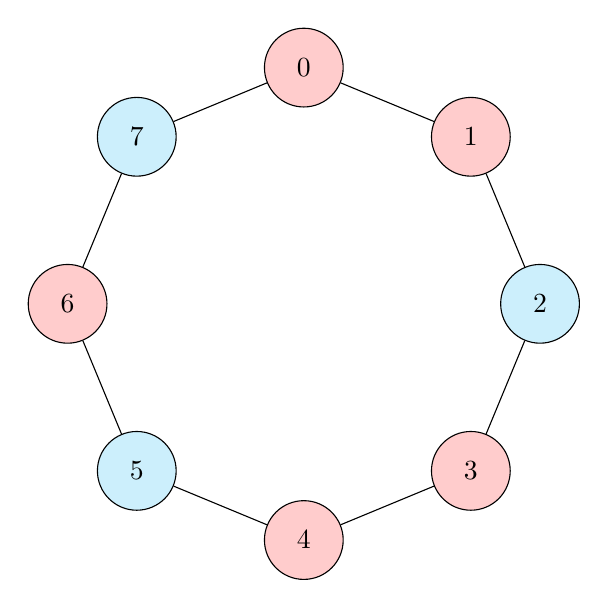
\begin{tikzpicture}

        % Define the number of circles and the radius of the ring
        \def\n{8}
        \def\radius{3}
        
        % Loop to draw the circles in a ring and add labels
        \foreach \i in {0,...,7} {
            \pgfmathsetmacro{\angle}{90 - \i * 360 / \n}
            \ifnum\i=0 \node[circle, draw, fill=red!20, minimum size=1cm] (C\i) at (\angle:\radius) {\i};
            \else\ifnum\i=1 \node[circle, draw, fill=red!20, minimum size=1cm] (C\i) at (\angle:\radius) {\i};
            \else\ifnum\i=3 \node[circle, draw, fill=red!20, minimum size=1cm] (C\i) at (\angle:\radius) {\i};
            \else\ifnum\i=4 \node[circle, draw, fill=red!20, minimum size=1cm] (C\i) at (\angle:\radius) {\i};
            \else\ifnum\i=6 \node[circle, draw, fill=red!20, minimum size=1cm] (C\i) at (\angle:\radius) {\i};
            \else\ifnum\i=2 \node[circle, draw, fill=cyan!20, minimum size=1cm] (C\i) at (\angle:\radius) {\i};
            \else\ifnum\i=5 \node[circle, draw, fill=cyan!20, minimum size=1cm] (C\i) at (\angle:\radius) {\i};
            \else \node[circle, draw, fill=cyan!20, minimum size=1cm] (C\i) at (\angle:\radius) {\i};
            \fi\fi\fi\fi\fi\fi\fi
        }
        
        % Loop to draw round links between each pair of adjacent circles
        \foreach \i in {0,...,7} {
            \pgfmathtruncatemacro{\nexti}{mod(\i+1,8)}
            \draw [rounded corners] (C\i) -- (C\nexti);
        }
        
        \end{tikzpicture}
    \caption{Chord ring with 8 nodes. Blue nodes represent data items, while red nodes represent Chord nodes.}
    \label{fig:chord-ring-nodes-entities}
\end{figure}

\section{Finger Tables}
For peers in a Chord network to locate each other, each peer must be aware of at least one other peer in the network.
Specifically, each peer needs to know the IP address (along with the TCP or UDP port) of their nearest neighbor in terms of identifier in the Chord network.
\begin{figure}[htbp]
    \centering
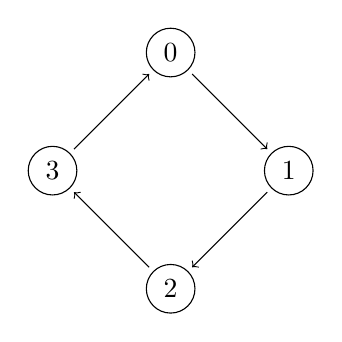
\begin{tikzpicture}
    % Define the positions of the nodes in a ring with shorter arrows
    \node[circle, draw] (0) at (90:1.5) {0};
    \node[circle, draw] (1) at (0:1.5) {1};
    \node[circle, draw] (2) at (270:1.5) {2};
    \node[circle, draw] (3) at (180:1.5) {3};
    
    % Draw the directional arrows between the nodes with shorter distances
    \draw[->, shorten >=2pt, shorten <=2pt] (0) -- (1);
    \draw[->, shorten >=2pt, shorten <=2pt] (1) -- (2);
    \draw[->, shorten >=2pt, shorten <=2pt] (2) -- (3);
    \draw[->, shorten >=2pt, shorten <=2pt] (3) -- (0);
\end{tikzpicture}
\caption{Chord ring with 4 nodes. Each node is aware of its immediate neighbors.}
\label{fig:chord-ring-peer-neighbours}
\end{figure}

This is illustrated in the Fig. \ref{fig:chord-ring-peer-neighbours}, where each node is aware of its immediate neighbors.

By knowing only the nearest neighboring peer in the network, it is still possible to find any peer.
The lookup algorithm works as follows:
\begin{enumerate}
    \item If the nearest neighbor is the peer (ID) we are looking for, the lookup is successful;
	\item Else, ask the nearest neighbor to return either the address of the target peer or the closest peer it knows to the target peer, if it doesn't know the target peer itself;
	\begin{itemize}
        \item If the returned peer (ID) is the peer we are looking for, the lookup is successful.
        \item If the neighboring peer does not know any peer closer to the target peer than itself, it returns no peer info, and the lookup is unsuccessful.
        \item Else, repeat step 2 by sending the request to the peer returned from the previous lookup request.
    \end{itemize}
\end{enumerate}

Using this simple algorithm, the searching peer will eventually query all peers in the network, one at a time, until it finds the target peer or concludes that the closest peer it knows is itself, which will occur after a complete round in the network.

However, only relying on the nearest neighbor results in a lookup time of $\mathcal{O}(N)$, meaning the lookup time increases linearly with the number of peers in the Chord network.
Chord addresses this problem with a more efficient solution.
\\To improve lookup times, the Chord finger table (also called routing table) is structured so that each peer maintains pointers (entries) to more than just their nearest neighbor in the Chord network.
The finger table of a node \(n\) contains up to \(m\) entries, where \(m\) is the number of bits in the identifier.
The $i-$th entry in the finger table of node \(n\) points to the first node that succeeds \(n + 2^{i-1}\) on the identifier circle.
This allows nodes to efficiently route queries by skipping intermediate nodes and reducing the number of hops (\cite{stoica2001}).
In other words, finger tables accelerate the lookup process in a Chord \gls{dht} by containing shortcuts to existing nodes in the ring, thereby reducing the distance traveled during the search for a particular node.
Each node has a finger table with the addresses of $m$ successive nodes, which is used to navigate to other nodes during lookup.
Here are some syntactical details of these finger tables commonly used in Chord \gls{dht} algorithms:
\begin{itemize}
    \item $FT_n$ represents the finger table for node $n$.
    For example, $FT_1$ refers to the finger table of node 1.
	\item $FT_n[i]$ represents the $i$-th successor of node $n$.
    For example, $FT_1[2]$ refers to the second successor node in the finger table of node 1.
\end{itemize}
Table \ref{tab:peer-finger-table} shows $FT_3$, the finger table for a peer with ID 3 in a Chord network with 8-bit IDs.
\begin{table}[htbp]
    \centering
    \begin{tabular}{|c|c|c|}
        \hline
        \textbf{Entry Index} & \textbf{Referenced ID} & \textbf{ID Distance} \\ \hline
        0 & 4 & $1 \ (2^0)$ \\ \hline
        1 & 5 & $2 \ (2^1)$ \\ \hline
        2 & 7 & $4 \ (2^2)$ \\ \hline
        3 & 11 & $8 \ (2^3)$ \\ \hline
        4 & 19 & $16 \ (2^4)$ \\ \hline
        5 & 35 & $32 \ (2^5)$ \\ \hline
        6 & 67 & $64 \ (2^6)$ \\ \hline
        7 & 131 & $128 \ (2^7)$ \\ \hline
    \end{tabular}
    \caption{A peer finger table for peer with ID 3 (8 bit ID size).}
    \label{tab:peer-finger-table}
\end{table}

The first 4 references of the peer with ID 3 are illustrated in Fig. \ref{fig:chord-ring-16-peers-4-references-peer-3}.
It provides a sense of how the exponentially increasing distances of references appear in a virtual Chord ring:

\begin{figure}[htbp]
    \centering
    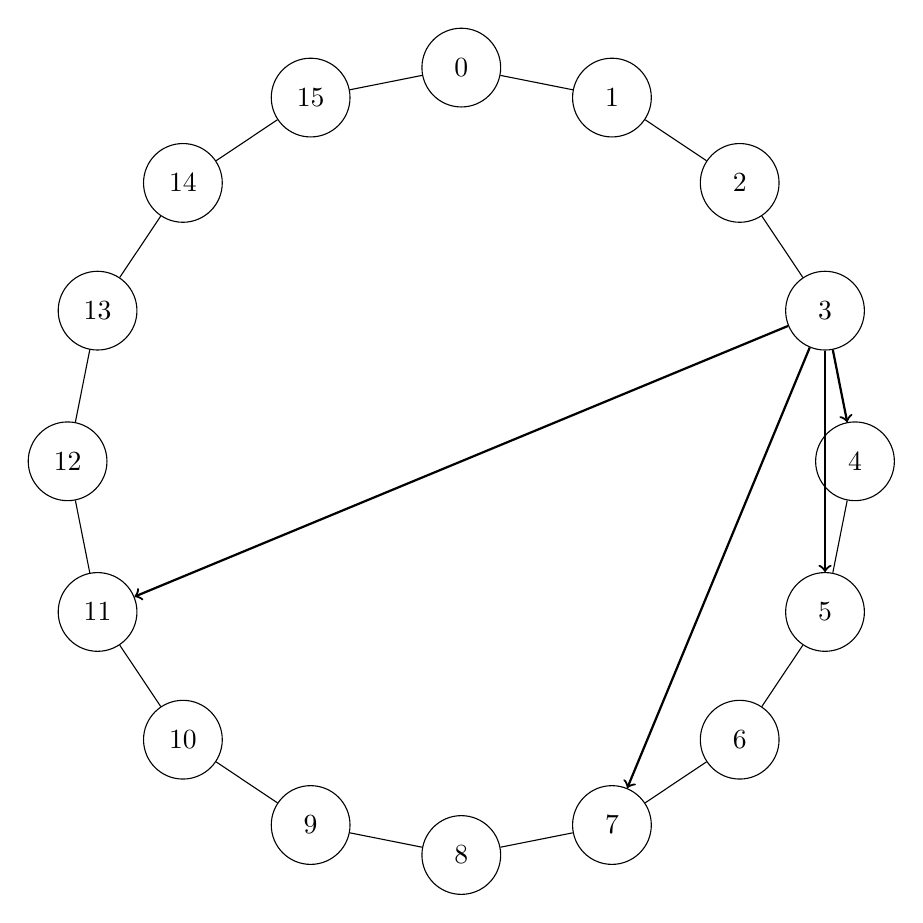
\begin{tikzpicture}

        % Define the number of circles and the radius of the ring
        \def\n{16}
        \def\radius{5}
        
        % Loop to draw the circles in a ring and add labels
        \foreach \i in {0,...,15} {
            \pgfmathsetmacro{\angle}{90 - \i * 360 / \n}
            \node[circle, draw, fill=white, minimum size=1cm] (C\i) at (\angle:\radius) {\i};
        }
        
        % Loop to draw round links between each pair of adjacent circles
        \foreach \i in {0,...,15} {
            \pgfmathtruncatemacro{\nexti}{mod(\i+1,16)}
            \draw [rounded corners] (C\i) -- (C\nexti);
        }

        % Draw additional directional arrows from node 3 to nodes 4, 5, 7, and 11
        \draw[->, thick] (C3) -- (C4);
        \draw[->, thick] (C3) -- (C5);
        \draw[->, thick] (C3) -- (C7);
        \draw[->, thick] (C3) -- (C11);
        
    \end{tikzpicture}
    \caption{Chord ring with 16 peers. The first 4 references of the peer with ID 3 are represented by the arrows.}
    \label{fig:chord-ring-16-peers-4-references-peer-3}
\end{figure}

\section{Lookups and Routing}
As explained in the previous section, when a node needs to locate a data item, it generates the identifier for the item using the hash function $H$.
The node then uses its finger table to forward the query to the appropriate node responsible for the identifier.
This process continues iteratively, with each node forwarding the query closer to the target node, until the node responsible for the data item is found.
The expected number of hops for a lookup is \(O(\log N)\) (\cite{stoica2001}).

\section{Chord Lookup Example}
To better understand how the Chord lookup algorithm works, let's examine a lookup example.
In this scenario, the peer with ID 3 needs to locate the peer with ID 2.

Firstly, here are the finger tables for the peers involved in this specific lookup (peers 3, 11, 15, and 1):
\begin{figure}[htbp]
    \centering
    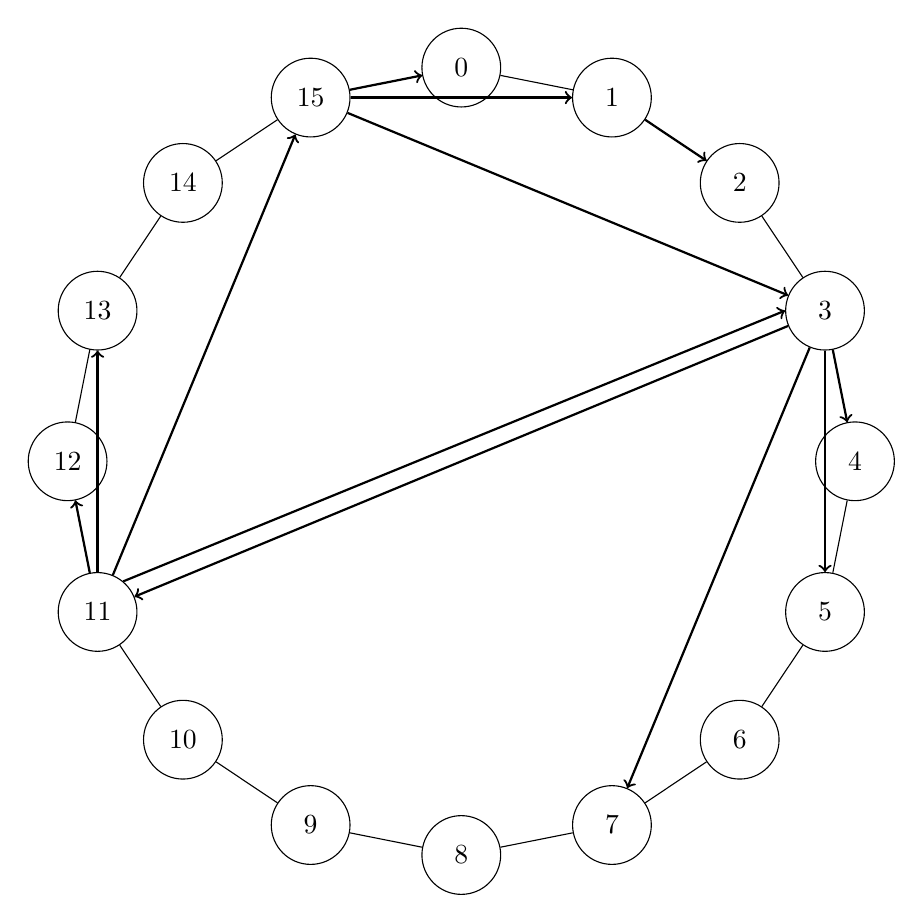
\begin{tikzpicture}

        % Define the number of circles and the radius of the ring
        \def\n{16}
        \def\radius{5}
        
        % Loop to draw the circles in a ring and add labels
        \foreach \i in {0,...,15} {
            \pgfmathsetmacro{\angle}{90 - \i * 360 / \n}
            \node[circle, draw, fill=white, minimum size=1cm] (C\i) at (\angle:\radius) {\i};
        }
        
        % Loop to draw round links between each pair of adjacent circles
        \foreach \i in {0,...,15} {
            \pgfmathtruncatemacro{\nexti}{mod(\i+1,16)}
            \draw [rounded corners] (C\i) -- (C\nexti);
        }

        % Draw additional directional arrows from node 3 to nodes 4, 5, 7, and 11
        \draw[->, thick] (C3) -- (C4);
        \draw[->, thick] (C3) -- (C5);
        \draw[->, thick] (C3) -- (C7);
        \draw[->, thick] (C3) -- (C11);
        \draw[->, thick] (C11) -- (C12);
        \draw[->, thick] (C11) -- (C13);
        \draw[->, thick] (C11.50) -- (C3.180);
        \draw[->, thick] (C11) -- (C15);
        \draw[->, thick] (C15) -- (C0);
        \draw[->, thick] (C15) -- (C1);
        \draw[->, thick] (C15) -- (C3);
        \draw[->, thick] (C1) -- (C2);
        
    \end{tikzpicture}
    \caption{Chord lookup example.}
    \label{fig:chord-ring-16-peers-lookup-example}
\end{figure}

The lookup process proceeds as follows:
\begin{enumerate}
    \item The peer with ID 3 first examines its own finger table and identifies the peer with the closest ID to 2, which is the peer with ID 11;
	\item The searching peer then contacts the peer with ID 11 and inquires about the closest peer it knows to the peer with ID 2. The peer with ID 11 points to the peer with ID 15;
	\item Next, the searching peer contacts the peer with ID 15 and asks for the closest peer it knows to the peer with ID 2. The peer with ID 15 points to the peer with ID 1;
	\item The searching peer then contacts the peer with ID 1 and asks for the closest peer it knows to the peer with ID 2. The peer with ID 1 points to the peer with ID 2.
\end{enumerate}

The lookup is now complete.

These steps are illustrated in Fig. \ref{fig:chord-example-lookup-steps}. The red arrows indicate the lookup progression.

\begin{figure}[htbp]
    \centering
    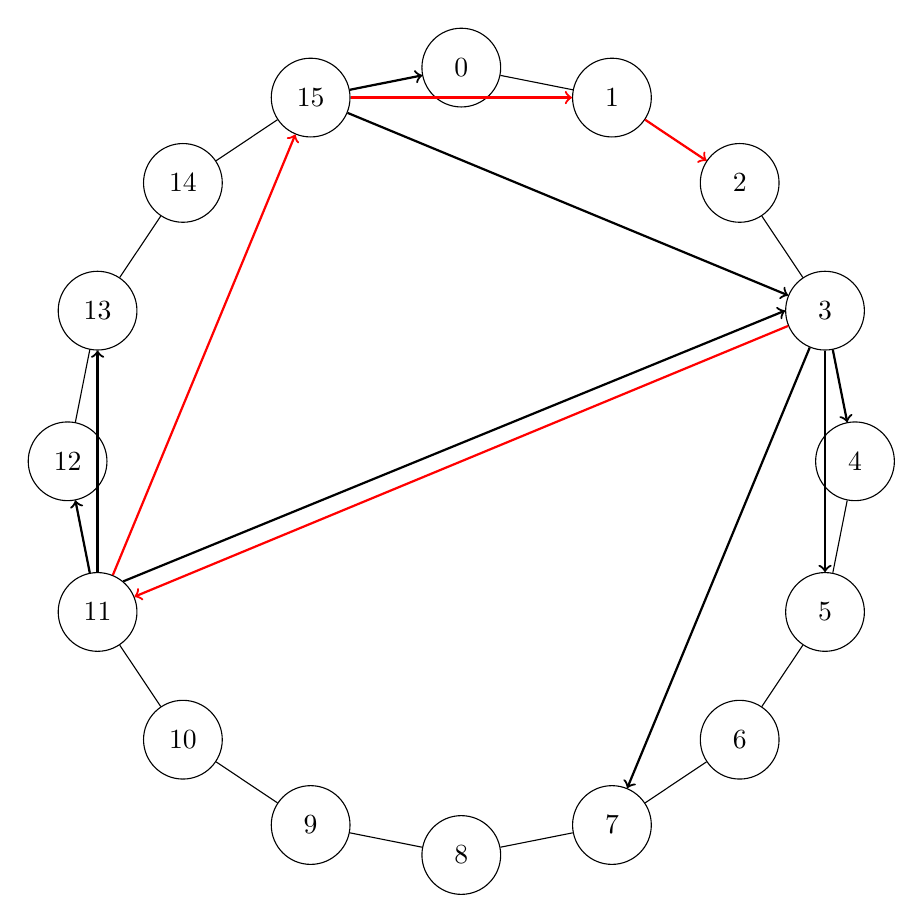
\begin{tikzpicture}

        % Define the number of circles and the radius of the ring
        \def\n{16}
        \def\radius{5}
        
        % Loop to draw the circles in a ring and add labels
        \foreach \i in {0,...,15} {
            \pgfmathsetmacro{\angle}{90 - \i * 360 / \n}
            \node[circle, draw, fill=white, minimum size=1cm] (C\i) at (\angle:\radius) {\i};
        }
        
        % Loop to draw round links between each pair of adjacent circles
        \foreach \i in {0,...,15} {
            \pgfmathtruncatemacro{\nexti}{mod(\i+1,16)}
            \draw [rounded corners] (C\i) -- (C\nexti);
        }

        % Draw additional directional arrows from node 3 to nodes 4, 5, 7, and 11
        \draw[->, thick] (C3) -- (C4);
        \draw[->, thick] (C3) -- (C5);
        \draw[->, thick] (C3) -- (C7);
        \draw[->, thick, red] (C3) -- (C11);
        \draw[->, thick] (C11) -- (C12);
        \draw[->, thick] (C11) -- (C13);
        \draw[->, thick] (C11.50) -- (C3.180);
        \draw[->, thick, red] (C11) -- (C15);
        \draw[->, thick] (C15) -- (C0);
        \draw[->, thick, red] (C15) -- (C1);
        \draw[->, thick] (C15) -- (C3);
        \draw[->, thick, red] (C1) -- (C2);
        
    \end{tikzpicture}
    \caption{Example of Chord lookup steps.}
    \label{fig:chord-example-lookup-steps}
\end{figure}

\section{Joining and Leaving the Network}
When a new node joins the Chord network, it must integrate into the existing structure.
The joining node needs to initialize its finger table and notify other nodes of its presence.
This involves updating the finger tables of existing nodes to reflect the new node's position.
The new node first contacts an existing node in the network to find its appropriate position in the identifier circle.
Once its position is determined, the new node initializes its finger table by querying other nodes for the necessary information.

The joining process also requires the new node to transfer relevant data from its predecessor, ensuring that data responsibility is correctly assigned.
Additionally, the new node must notify its predecessor and successor about its presence, prompting them to update their respective finger tables.
This notification process may propagate further updates across the network to maintain the integrity and efficiency of the lookup process.

When a node leaves the network, it must transfer its data to its successor node and notify other nodes to update their finger tables accordingly.
The departing node first ensures that all its data is transferred to its immediate successor, guaranteeing no data loss occurs.
Following the data transfer, the leaving node informs its predecessor and successor, as well as potentially other nodes, to adjust their finger tables to exclude the departing node.

Chord's protocol is designed to handle frequent join and leave operations seamlessly, ensuring the network remains robust and efficient.
This self-healing capability of the Chord network allows it to maintain consistent data availability and efficient routing performance.
The protocol dynamically adjusts the finger tables and data responsibilities, minimizing the impact of node churn on the overall system.

Furthermore, Chord uses stabilization protocols that periodically run to correct any inconsistencies in the finger tables and ensure all nodes have accurate and up-to-date routing information.
These stabilization routines help in maintaining the correctness and performance of the network despite the continuous changes in its composition.

By effectively managing the joining and leaving of nodes, Chord ensures that the \gls{dht} structure remains functional, providing a scalable and resilient platform for distributed applications.

Chord's ability to adapt to the dynamic nature of \gls{p2p} networks, where nodes frequently join and leave, highlights its efficiency and reliability.
The protocol's mechanisms for updating finger tables and redistributing data ensure that the network can sustain a high degree of availability and performance, which are crucial for the practical deployment of distributed systems (\cite{stoica2001}).

\section{Advantages and Limitations}
One of the primary advantages of Chord is its scalability.
The protocol can efficiently manage a large number of nodes, ensuring that as the number of nodes grows, the number of steps required to find a particular data item increases logarithmically.
This property makes Chord highly suitable for applications requiring dynamic and scalable networks, such as \gls{p2p} systems (\cite{stoica2001}).
Additionally, Chord provides a decentralized approach, eliminating the need for a central coordinator, which enhances fault tolerance and reduces single points of failure.
Each node in the network maintains only a small amount of routing information about other nodes, enabling the network to handle frequent node arrivals and departures without significant disruptions.

Another advantage of Chord is its simplicity and ease of implementation.
The protocol relies on consistent hashing to distribute data across nodes uniformly, which simplifies the process of locating and retrieving data.
This uniform distribution helps in balancing the load among nodes, preventing any single node from becoming a bottleneck (\cite{stoica2001}).
Moreover, Chord's ring structure allows for efficient data retrieval, as each node only needs to know about its successor and a few other nodes in the ring to route queries effectively.

However, Chord also has several disadvantages.
One significant limitation is its reliance on consistent hashing, which, while effective in balancing load, can lead to suboptimal data placement and increased latency in certain scenarios.
For example, if the hash function does not evenly distribute data, some nodes may end up handling more requests than others, leading to uneven load distribution and potential performance bottlenecks (\cite{stoica2001}).
Additionally, Chord's performance can be impacted by network latency and the physical distribution of nodes, as the protocol does not consider the proximity of nodes when routing queries, potentially resulting in longer query times (\cite{balatsouras2022wichord}).

Another disadvantage of Chord is its maintenance overhead.
As nodes frequently join and leave the network, the protocol must constantly update its routing information to maintain consistency and ensure efficient data retrieval.
This maintenance can introduce additional communication overhead and complexity, particularly in highly dynamic environments (\cite{stoica2001}).
Furthermore, while Chord is designed to be fault-tolerant, it still requires mechanisms to handle node failures and recover lost data, which can add to the system's overall complexity and resource requirements.

In conclusion, while the Chord protocol offers significant advantages in terms of scalability, decentralization, and simplicity, it also faces challenges related to data placement, network latency, and maintenance overhead.
These factors must be carefully considered when implementing Chord in distributed systems to ensure optimal performance and reliability.